%\addtocounter{chapter}{3}%only temporary
\chapter{DSA Procedure Using GALS}\label{sec:algo}
Bla Bla

\begin{figure}[!htb]
\begin{center}
%\hspace{35mm}
%\vspace{3mm}
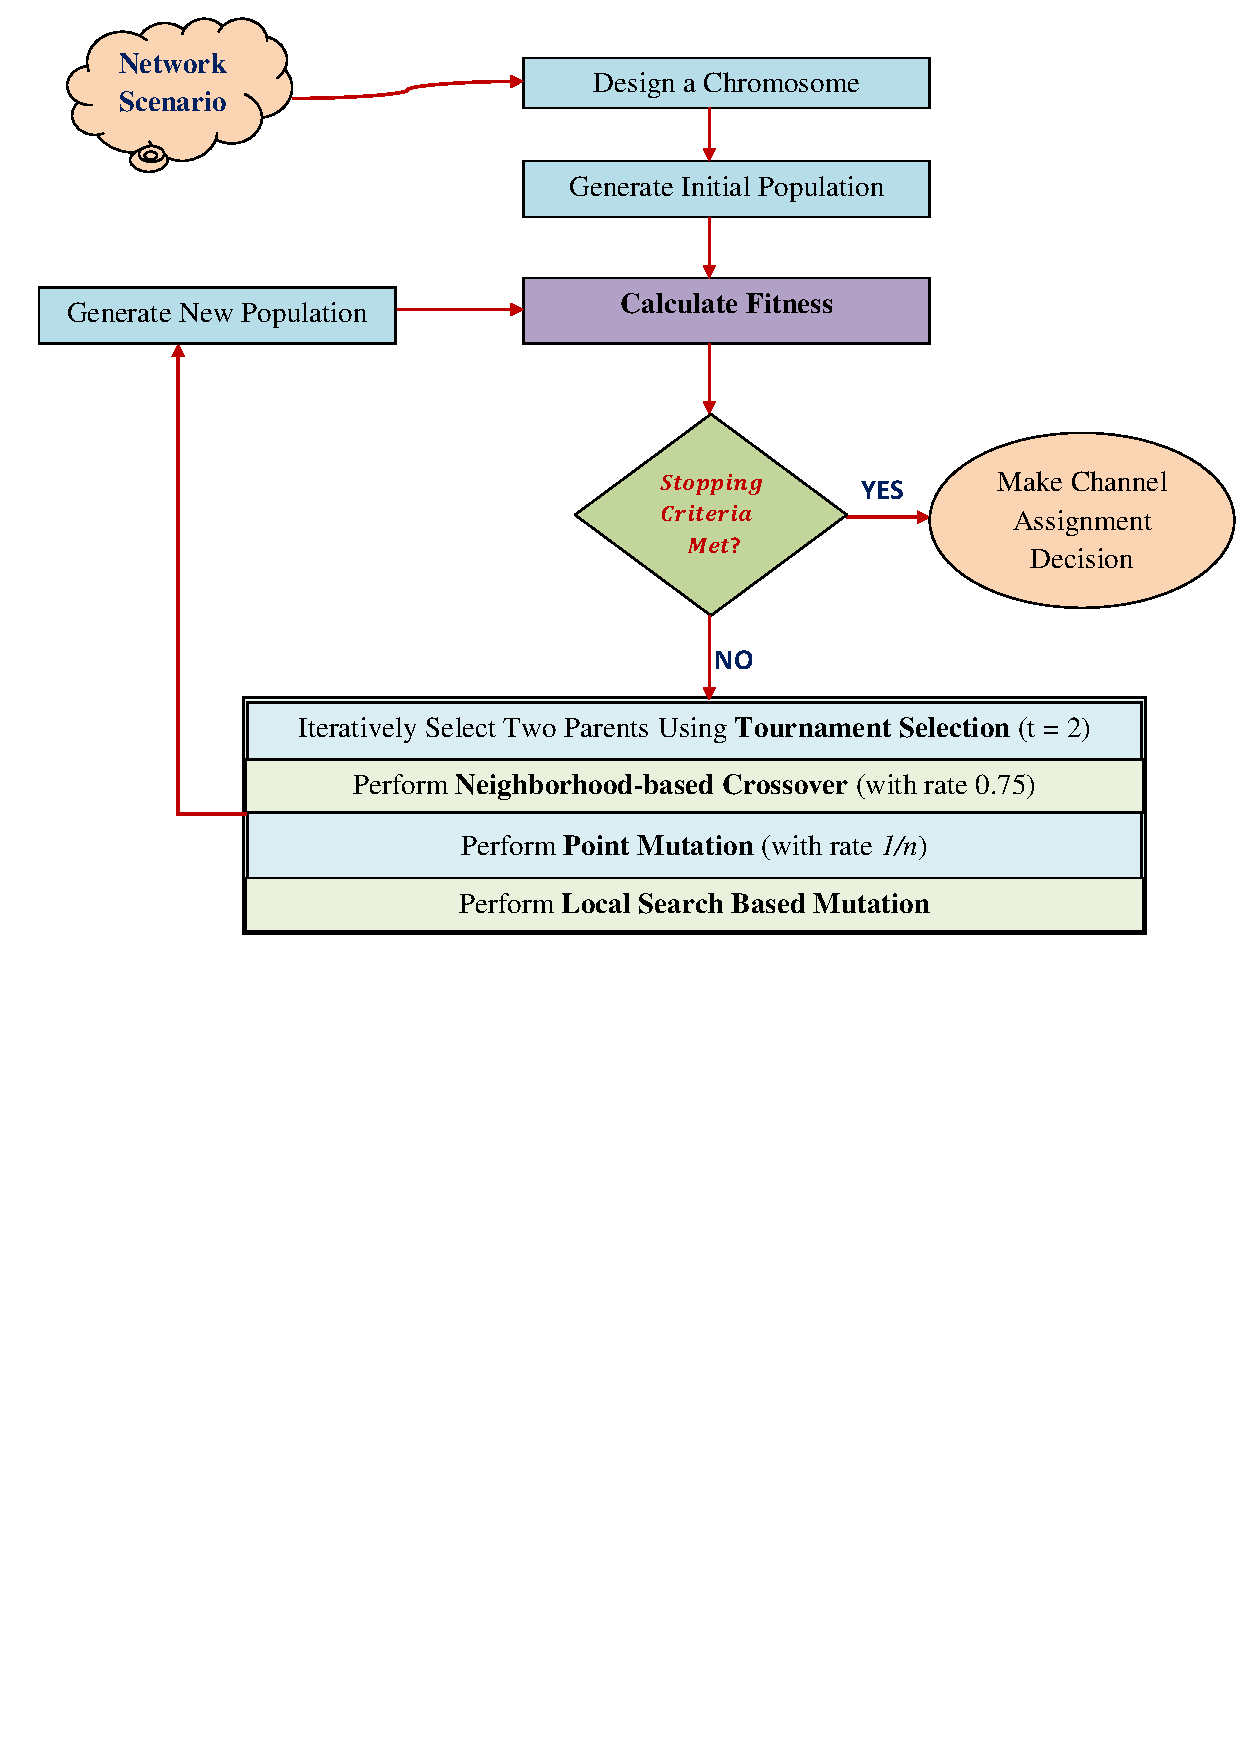
\includegraphics [scale=0.8]{algos/GALS.pdf}
\vspace{-106mm}
\caption{Algorithmic structure of GALS}
\vspace{-3mm}
\label{GALSalgo}
\end{center}
\end{figure}


 
%\vspace{-2mm}
\begin{center}
%\vspace{-3mm}
\begin{algorithm}[!thb]
%\SetAlgoLined
%\SetKwInOut{Procedure: GALS}{Procedure: GALS}
%\SetKwInOut{Begin}{Begin} \SetKwInOut{End}{End}
%\SetKwInOut{Data:}{Data:} \SetKwInOut{Parameter settings:}{Parameter settings:}
%\textbf{Procedure: GALS{}}
\BlankLine
\textit{begin{}}
\BlankLine
\If{there is an unused channel $cl$}
{
	Select $cl$ and \Return\\
}
Initialize parameters\\
Generate initial population $\varphi$ \\
$generation \leftarrow 1$ \\
\BlankLine
\While {generation $\le$ $M_T$ \& global optima not reached}
{
	Initialize new population $\varphi_{new}=null$ \\
	Calculate fitness of each individual of $\varphi$\\
	Set $S \leftarrow null$\\
	\While {$|\varphi_{new}| < |\varphi|$}
	{
		Select two parents from $\varphi$ using tournament \qquad selection (t = 2) \\
		Add the parents to $S$\\
%		Choose a random number $r \in [0, 1]$ \\
%		\If {$r \le \alpha_c$}
%        {
    	  Perform neighborhood-based crossover (rate $\alpha_c$)\\
%        }
%       \Else
%	   {
%		  Perform 2-point crossover\\
%	   } 
		
		Perform point mutation (rate $\alpha_m$) \\
		Add the generated off-springs to $S$ \\

		$a \leftarrow$  a random individual in $S$ \\
		Remove $a$ from $S$ and add to $\varphi_{new}$ \\

		\ForEach{individual in $S$}
		{
		   Perform local search based mutation \\
		   Calculate fitness \\	
		}

		$b \leftarrow$  the best individual in $S$ \\
		Add $b$ to $\varphi_{new}$\\		 
	}
	$generation \leftarrow generation + 1$\\
	$\varphi \leftarrow \varphi_{new}$ \\
}
\BlankLine
Sort the individuals according to their fitness values \\
\textit{solution} $\leftarrow$ the best individual of $\varphi$ \\
$u_r \leftarrow$ own user ID \\
$c \leftarrow$ value at $u_r^{th}$ position of the \textit{solution}\\
Select channel $c$ for $u_r$ \\
\Return \\
\BlankLine
\textit{end{}}
\vspace{2mm}
\caption{Channel assignment in GALS}
\label{alg:algo}
\end{algorithm}
\vspace{3mm}
\end{center}



\section{Computational Complexity}
Bla Bla

\subsection{Per-iteration Time Complexity}
Bla Bla

\begin{equation*}
%\vspace{-10mm}
\begin{split}
T(n, m) &\Rightarrow O(m+n |\varphi|) + O(M_T(|\varphi|(n+m)+t+n+m)) + O( |\varphi|\log(|\varphi|) + 1) \\
&\Rightarrow  O(m) + O(n+m) \\
& \Rightarrow O(n+m)
\end{split}
\end{equation*}



\vspace{3mm}
\subsection{Space Complexity}
Bla Bla
%\vspace{-5mm}
\begin{equation*}
\begin{split}
S(n, m) & \Rightarrow O(m+nm) + O(2n |\varphi|) + O(n) \\ 
& \Rightarrow O(nm) + O(n) \\ 
& \Rightarrow O(nm)
\end{split}
\end{equation*}
\vspace{2mm}
